\documentclass[12pt]{article} 
\usepackage[margin=2cm]{geometry} 
\usepackage{psfrag} 
\usepackage{graphicx} 
\usepackage{epstopdf} 
\usepackage{longtable,booktabs} 
\usepackage{amsmath,amsfonts} 
\usepackage{breqn} 
\usepackage{float,morefloats,caption} 
\begin{document} 
% 22-Mar-2024 15:49:13, created by stoch_simul.m 
 
\begin{center}
\begin{longtable}{lcc} 
\caption{MATRIX OF COVARIANCE OF EXOGENOUS SHOCKS}\\
 \label{Table:covar_ex_shocks}\\
\toprule 
$Variables       $	 & 	 $   {\epsilon^{A}}$	 & 	 $   {\epsilon^{G}}$\\
\midrule \endfirsthead 
\caption{(continued)}\\
 \toprule \\ 
$Variables       $	 & 	 $   {\epsilon^{A}}$	 & 	 $   {\epsilon^{G}}$\\
\midrule \endhead 
\midrule \multicolumn{3}{r}{(Continued on next page)} \\ \bottomrule \endfoot 
\bottomrule \endlastfoot 
${\epsilon^{A}}  $	 & 	          1.000000	 & 	          0.000000 \\ 
${\epsilon^{G}}  $	 & 	          0.000000	 & 	          1.000000 \\ 
\end{longtable}
 \end{center}
% End of TeX file.
 
\begin{center}
\begin{longtable}{ccc}
\caption{Endogenous}\\%
\hline%
\multicolumn{1}{c}{\textbf{Variable}} &
\multicolumn{1}{c}{\textbf{\LaTeX}} &
\multicolumn{1}{c}{\textbf{Description}}\\%
\hline\hline%
\endfirsthead
\multicolumn{3}{c}{{\tablename} \thetable{} -- Continued}\\%
\hline%
\multicolumn{1}{c}{\textbf{Variable}} &
\multicolumn{1}{c}{\textbf{\LaTeX}} &
\multicolumn{1}{c}{\textbf{Description}}\\%
\hline\hline%
\endhead
\texttt{uc} & $U^{C}$ & Marginal utility of consumption\\
\texttt{ul} & $U^{L}$ & Marginal utility of labour\\
\texttt{r} & $R$ & Risk free interest rate\\
\texttt{h} & $H$ & Hours\\
\texttt{w} & $W$ & Real wage\\
\texttt{y} & $Y$ & Output\\
\texttt{k} & $K$ & Capital\\
\texttt{i} & $I$ & Investment\\
\texttt{c} & $C$ & Consumption\\
\texttt{a} & $A$ & Technology\\
\texttt{g} & $G$ & Government spending\\
\hline%
\end{longtable}
\end{center}
\begin{center}
\begin{longtable}{ccc}
\caption{Exogenous}\\%
\hline%
\multicolumn{1}{c}{\textbf{Variable}} &
\multicolumn{1}{c}{\textbf{\LaTeX}} &
\multicolumn{1}{c}{\textbf{Description}}\\%
\hline\hline%
\endfirsthead
\multicolumn{3}{c}{{\tablename} \thetable{} -- Continued}\\%
\hline%
\multicolumn{1}{c}{\textbf{Variable}} &
\multicolumn{1}{c}{\textbf{\LaTeX}} &
\multicolumn{1}{c}{\textbf{Description}}\\%
\hline\hline%
\endhead
\texttt{epsA} & ${\epsilon^{A}}$ & Labor Augmenting shock\\
\texttt{epsG} & ${\epsilon^{G}}$ & Government Spending shock\\
\hline%
\end{longtable}
\end{center}
\begin{center}
\begin{longtable}{ccc}
\caption{Parameters}\\%
\hline%
\multicolumn{1}{c}{\textbf{Variable}} &
\multicolumn{1}{c}{\textbf{\LaTeX}} &
\multicolumn{1}{c}{\textbf{Description}}\\%
\hline\hline%
\endfirsthead
\multicolumn{3}{c}{{\tablename} \thetable{} -- Continued}\\%
\hline%
\multicolumn{1}{c}{\textbf{Variable}} &
\multicolumn{1}{c}{\textbf{\LaTeX}} &
\multicolumn{1}{c}{\textbf{Description}}\\%
\hline\hline%
\endhead
\texttt{varrho} & ${\varrho}$ & Weight on Leisure in utility\\
\texttt{alp} & ${\alpha}$ & Labour share\\
\texttt{betta} & ${\beta}$ & Discount factor\\
\texttt{delta} & ${\delta}$ & Capital depreciation\\
\texttt{sigma\_c} & ${\sigma_{C}}$ & Inverse of the elasticity of substitution\\
\texttt{cy} & $\frac{\bar{C}}{\bar{Y}}$ & Consumption output ratio in steady state\\
\texttt{iy} & $\frac{\bar{I}}{\bar{Y}}$ & Investment output ratio in steady state\\
\texttt{gy} & $\frac{\bar{G}}{\bar{Y}}$ & Government output ratio\\
\texttt{H\_bar} & $\bar{H}$ & Steady state hours\\
\texttt{R\_bar} & $\bar{R}$ & Steady state risk free interest rate\\
\texttt{A\_bar} & $\bar{A}$ & Steady state technology\\
\texttt{rhoA} & ${\rho_{A}}$ & Persistence of labor augmentig shock\\
\texttt{rhoG} & ${\rho_{G}}$ & Persistence of government spending shock\\
\texttt{sigma} & ${\sigma}$ & Shock scaling parameter\\
\hline%
\end{longtable}
\end{center}
 
\begin{center}
\begin{longtable}{ccc}
\caption{Parameter Values}\\%
\toprule%
\multicolumn{1}{c}{\textbf{Parameter}} &
\multicolumn{1}{c}{\textbf{Value}} &
 \multicolumn{1}{c}{\textbf{Description}}\\%
\midrule%
\endfirsthead
\multicolumn{3}{c}{{\tablename} \thetable{} -- Continued}\\%
\midrule%
\multicolumn{1}{c}{\textbf{Parameter}} &
\multicolumn{1}{c}{\textbf{Value}} &
  \multicolumn{1}{c}{\textbf{Description}}\\%
\midrule%
\endhead
${\varrho}$ 	 & 	 0.689 	 & 	 Weight on Leisure in utility\\
${\alpha}$ 	 & 	 0.700 	 & 	 Labour share\\
${\beta}$ 	 & 	 0.990 	 & 	 Discount factor\\
${\delta}$ 	 & 	 0.025 	 & 	 Capital depreciation\\
${\sigma_{C}}$ 	 & 	 2.000 	 & 	 Inverse of the elasticity of substitution\\
$\frac{\bar{C}}{\bar{Y}}$ 	 & 	 0.586 	 & 	 Consumption output ratio in steady state\\
$\frac{\bar{I}}{\bar{Y}}$ 	 & 	 0.214 	 & 	 Investment output ratio in steady state\\
$\frac{\bar{G}}{\bar{Y}}$ 	 & 	 0.200 	 & 	 Government output ratio\\
$\bar{H}$ 	 & 	 0.350 	 & 	 Steady state hours\\
$\bar{R}$ 	 & 	 1.010 	 & 	 Steady state risk free interest rate\\
$\bar{A}$ 	 & 	 1.000 	 & 	 Steady state technology\\
${\rho_{A}}$ 	 & 	 0.750 	 & 	 Persistence of labor augmentig shock\\
${\rho_{G}}$ 	 & 	 0.750 	 & 	 Persistence of government spending shock\\
${\sigma}$ 	 & 	 1.000 	 & 	 Shock scaling parameter\\
\bottomrule%
\end{longtable}
\end{center}
 
% 22-Mar-2024 15:49:13, created by disp_th_moments.m 
 
\begin{center}
\begin{longtable}{lccccc} 
\caption{COEFFICIENTS OF AUTOCORRELATION}\\
 \label{Table:th_autocorr_matrix}\\
\toprule 
$Order   $	 & 	 $         1$	 & 	 $         2$	 & 	 $         3$	 & 	 $         4$	 & 	 $         5$\\
\midrule \endfirsthead 
\caption{(continued)}\\
 \toprule \\ 
$Order   $	 & 	 $         1$	 & 	 $         2$	 & 	 $         3$	 & 	 $         4$	 & 	 $         5$\\
\midrule \endhead 
\midrule \multicolumn{6}{r}{(Continued on next page)} \\ \bottomrule \endfoot 
\bottomrule \endlastfoot 
$Y       $	 & 	    0.7750	 & 	    0.6052	 & 	    0.4769	 & 	    0.3798	 & 	    0.3061 \\ 
$C       $	 & 	    0.9471	 & 	    0.8995	 & 	    0.8562	 & 	    0.8165	 & 	    0.7797 \\ 
$I       $	 & 	    0.7294	 & 	    0.5274	 & 	    0.3766	 & 	    0.2643	 & 	    0.1807 \\ 
$H       $	 & 	    0.7181	 & 	    0.5079	 & 	    0.3515	 & 	    0.2354	 & 	    0.1495 \\ 
$W       $	 & 	    0.8631	 & 	    0.7559	 & 	    0.6711	 & 	    0.6034	 & 	    0.5485 \\ 
$R       $	 & 	    0.8138	 & 	    0.6717	 & 	    0.5626	 & 	    0.4784	 & 	    0.4130 \\ 
\end{longtable}
 \end{center}
% End of TeX file.
 
% 22-Mar-2024 15:49:13, created by disp_th_moments.m 
 
\begin{center}
\begin{longtable}{lcccccc} 
\caption{MATRIX OF CORRELATIONS}\\
 \label{Table:th_corr_matrix}\\
\toprule 
$Variables  $	 & 	 $         Y$	 & 	 $         C$	 & 	 $         I$	 & 	 $         H$	 & 	 $         W$	 & 	 $         R$\\
\midrule \endfirsthead 
\caption{(continued)}\\
 \toprule \\ 
$Variables  $	 & 	 $         Y$	 & 	 $         C$	 & 	 $         I$	 & 	 $         H$	 & 	 $         W$	 & 	 $         R$\\
\midrule \endhead 
\midrule \multicolumn{7}{r}{(Continued on next page)} \\ \bottomrule \endfoot 
\bottomrule \endlastfoot 
$Y          $	 & 	    1.0000	 & 	    0.7813	 & 	    0.9499	 & 	    0.8615	 & 	    0.9432	 & 	    0.4462 \\ 
$C          $	 & 	    0.7813	 & 	    1.0000	 & 	    0.6092	 & 	    0.3562	 & 	    0.9443	 & 	   -0.2080 \\ 
$I          $	 & 	    0.9499	 & 	    0.6092	 & 	    1.0000	 & 	    0.9265	 & 	    0.8252	 & 	    0.6308 \\ 
$H          $	 & 	    0.8615	 & 	    0.3562	 & 	    0.9265	 & 	    1.0000	 & 	    0.6439	 & 	    0.8373 \\ 
$W          $	 & 	    0.9432	 & 	    0.9443	 & 	    0.8252	 & 	    0.6439	 & 	    1.0000	 & 	    0.1246 \\ 
$R          $	 & 	    0.4462	 & 	   -0.2080	 & 	    0.6308	 & 	    0.8373	 & 	    0.1246	 & 	    1.0000 \\ 
\end{longtable}
 \end{center}
% End of TeX file.
 
% 22-Mar-2024 15:49:13, created by disp_th_moments.m 
 
\begin{center}
\begin{longtable}{lccc} 
\caption{THEORETICAL MOMENTS}\\
 \label{Table:th_moments}\\
\toprule 
$VARIABLE  $	 & 	 $         MEAN$	 & 	 $    STD. DEV.$	 & 	 $     VARIANCE$\\
\midrule \endfirsthead 
\caption{(continued)}\\
 \toprule \\ 
$VARIABLE  $	 & 	 $         MEAN$	 & 	 $    STD. DEV.$	 & 	 $     VARIANCE$\\
\midrule \endhead 
\midrule \multicolumn{4}{r}{(Continued on next page)} \\ \bottomrule \endfoot 
\bottomrule \endlastfoot 
$Y         $	 & 	       0.0000	 & 	       1.6553	 & 	       2.7400 \\ 
$C         $	 & 	       0.0000	 & 	       0.8994	 & 	       0.8090 \\ 
$I         $	 & 	       0.0000	 & 	       6.0990	 & 	      37.1980 \\ 
$H         $	 & 	       0.0000	 & 	       0.7187	 & 	       0.5165 \\ 
$W         $	 & 	       0.0000	 & 	       1.0985	 & 	       1.2067 \\ 
$R         $	 & 	       0.0000	 & 	       0.0452	 & 	       0.0020 \\ 
\end{longtable}
 \end{center}
% End of TeX file.
 
% 22-Mar-2024 15:49:13, created by disp_th_moments.m 
 
\begin{center}
\begin{longtable}{lcc} 
\caption{VARIANCE DECOMPOSITION (in percent)}\\
 \label{Table:th_var_decomp_uncond}\\
\toprule 
$   $	 & 	 $   {\epsilon^{A}}$	 & 	 $   {\epsilon^{G}}$\\
\midrule \endfirsthead 
\caption{(continued)}\\
 \toprule \\ 
$   $	 & 	 $   {\epsilon^{A}}$	 & 	 $   {\epsilon^{G}}$\\
\midrule \endhead 
\midrule \multicolumn{3}{r}{(Continued on next page)} \\ \bottomrule \endfoot 
\bottomrule \endlastfoot 
$Y  $	 & 	             99.92	 & 	              0.08 \\ 
$C  $	 & 	             97.64	 & 	              2.36 \\ 
$I  $	 & 	             96.99	 & 	              3.01 \\ 
$H  $	 & 	             98.50	 & 	              1.50 \\ 
$W  $	 & 	             99.26	 & 	              0.74 \\ 
$R  $	 & 	             97.16	 & 	              2.84 \\ 
\end{longtable}
 \end{center}
% End of TeX file.
 
% Equation 1
\begin{dmath}
{UCF}_{t}=\left(\left(1-{{\varrho}}\right)\, \left(1-{{\sigma_{C}}}\right)-1\right)\, \left(\frac{{CF}_{t}}{1-{{\chi}}}-\frac{{{\chi}}}{1-{{\chi}}}\, {CF}_{t-1}\right)+{{\varrho}}\, \left({{\sigma_{C}}}-1\right)\, \frac{{{\bar{H}}}}{1-{{\bar{H}}}}\, {HF}_{t}
\end{dmath}
% Equation 2
\begin{dmath}
{UCF}_{t+1}={UCF}_{t}-{RF}_{t}
\end{dmath}
% Equation 3
\begin{dmath}
{ULF}_{t}=\left(-{UCF}_{t}\right)-\left(\frac{{CF}_{t}}{1-{{\chi}}}-\frac{{{\chi}}}{1-{{\chi}}}\, {CF}_{t-1}\right)-\frac{{{\bar{H}}}}{1-{{\bar{H}}}}\, {HF}_{t}
\end{dmath}
% Equation 4
\begin{dmath}
{WF}_{t}=\left(-{ULF}_{t}\right)-{UCF}_{t}
\end{dmath}
% Equation 5
\begin{dmath}
{YF}_{t}={{\alpha}}\, \left({HF}_{t}+{A}_{t}\right)+\left(1-{{\alpha}}\right)\, {KF}_{t-1}
\end{dmath}
% Equation 6
\begin{dmath}
{WF}_{t}={YF}_{t}-{HF}_{t}
\end{dmath}
% Equation 7
\begin{dmath}
{YF}_{t}={CF}_{t}\, {{cyf}}+{{iyf}}\, {IF}_{t}+{{gy}}\, {GF}_{t}
\end{dmath}
% Equation 8
\begin{dmath}
{KF}_{t}={IF}_{t}\, {{\delta}}+{KF}_{t-1}\, \left(1-{{\delta}}\right)
\end{dmath}
% Equation 9
\begin{dmath}
{XF}_{t}=\frac{{{\delta}}+{{\bar{RF}}}-1}{{{\bar{RF}}}}\, \left({YF}_{t}-{KF}_{t-1}\right)+\frac{1-{{\delta}}}{{{\bar{RF}}}}\, {QF}_{t}
\end{dmath}
% Equation 10
\begin{dmath}
{RF}_{t}={XF}_{t+1}-{QF}_{t}
\end{dmath}
% Equation 11
\begin{dmath}
{IF}_{t}\, \left(1+\frac{1}{{{\bar{RF}}}}\right)=\frac{1}{{{\bar{RF}}}}\, {IF}_{t+1}+{IF}_{t-1}+{QF}_{t}\, \frac{1}{2\, {{\phi_{X}}}}
\end{dmath}
% Equation 12
\begin{dmath}
{GF}_{t}={HF}_{t}+{WF}_{t}+{TaxF}_{t}
\end{dmath}
% Equation 13
\begin{dmath}
{GF}_{t}={{\rho_{G}}}\, {GF}_{t-1}+{{\epsilon^{G}}}_{t}
\end{dmath}
% Equation 14
\begin{dmath}
{UC}_{t}=\left(\left(1-{{\varrho}}\right)\, \left(1-{{\sigma_{C}}}\right)-1\right)\, \left(\frac{{C}_{t}}{1-{{\chi}}}-\frac{{{\chi}}}{1-{{\chi}}}\, {C}_{t-1}\right)+{{\varrho}}\, \left({{\sigma_{C}}}-1\right)\, \frac{{{\bar{H}}}}{1-{{\bar{H}}}}\, {H}_{t}
\end{dmath}
% Equation 15
\begin{dmath}
{UC}_{t+1}={UC}_{t}-{R}_{t+1}
\end{dmath}
% Equation 16
\begin{dmath}
{UH}_{t}=\left(-{UC}_{t}\right)-\left(\frac{{C}_{t}}{1-{{\chi}}}-\frac{{{\chi}}}{1-{{\chi}}}\, {C}_{t-1}\right)-\frac{{{\bar{H}}}}{1-{{\bar{H}}}}\, {H}_{t}
\end{dmath}
% Equation 17
\begin{dmath}
{W}_{t}=\left(-{UH}_{t}\right)-{UC}_{t}
\end{dmath}
% Equation 18
\begin{dmath}
{Y}_{t}={{\alpha}}\, \left({A}_{t}+{H}_{t}\right)+\left(1-{{\alpha}}\right)\, {K}_{t-1}
\end{dmath}
% Equation 19
\begin{dmath}
{MC}_{t}={H}_{t}+{W}_{t}-{Y}_{t}
\end{dmath}
% Equation 20
\begin{dmath}
{Y}_{t}={C}_{t}\, {{cy}}+{{iy}}\, {I}_{t}+{{gy}}\, {G}_{t}
\end{dmath}
% Equation 21
\begin{dmath}
{K}_{t}={{\delta}}\, {I}_{t}+\left(1-{{\delta}}\right)\, {K}_{t-1}
\end{dmath}
% Equation 22
\begin{dmath}
{X}_{t}=\frac{{{\delta}}+{{\bar{R}}}-1}{{{\bar{R}}}}\, \left({Y}_{t}+{MC}_{t}-{K}_{t-1}\right)+\frac{1-{{\delta}}}{{{\bar{R}}}}\, {Q}_{t}
\end{dmath}
% Equation 23
\begin{dmath}
{R}_{t+1}={X}_{t+1}-{Q}_{t}
\end{dmath}
% Equation 24
\begin{dmath}
{I}_{t}\, \left(1+\frac{1}{{{\bar{R}}}}\right)=\frac{1}{{{\bar{R}}}}\, {I}_{t+1}+{I}_{t-1}+\frac{1}{2\, {{\phi_{X}}}}\, {Q}_{t}
\end{dmath}
% Equation 25
\begin{dmath}
{G}_{t}={H}_{t}+{W}_{t}+{Tax}_{t}
\end{dmath}
% Equation 26
\begin{dmath}
{Pi}_{t}=\frac{{{\beta}}}{1+{{\beta}}\, {{\gamma^{p}}}}\, {Pi}_{t+1}+\frac{{{\gamma^{p}}}}{1+{{\beta}}\, {{\gamma^{p}}}}\, {Pi}_{t-1}+\frac{\left(1-{{\beta}}\, {{\xi}}\right)\, \left(1-{{\xi}}\right)}{\left(1+{{\beta}}\, {{\gamma^{p}}}\right)\, {{\xi}}}\, \left({MC}_{t}+{MS}_{t}\right)
\end{dmath}
% Equation 27
\begin{dmath}
{Rn}_{t}={{\rho_{R}}}\, {Rn}_{t-1}+{Pi}_{t}\, \left(1-{{\rho_{R}}}\right)\, {\theta^{\pi}}+{Y}_{t}\, \left(1-{{\rho_{R}}}\right)\, {\theta^{y}}+{{\epsilon^{M}}}_{t}
\end{dmath}
% Equation 28
\begin{dmath}
{R}_{t}={Rn}_{t-1}-{Pi}_{t}
\end{dmath}
% Equation 29
\begin{dmath}
{E(R)}_{t}={Rn}_{t}-{Pi}_{t+1}
\end{dmath}
% Equation 30
\begin{dmath}
{A}_{t}={{\rho_{A}}}\, {A}_{t-1}+{{\epsilon^{A}}}_{t}
\end{dmath}
% Equation 31
\begin{dmath}
{G}_{t}={{\epsilon^{G}}}_{t}+{{\rho_{G}}}\, {G}_{t-1}
\end{dmath}
% Equation 32
\begin{dmath}
{MS}_{t}={{\rho_{MS}}}\, {MS}_{t-1}+{{\epsilon^{MS}}}_{t}
\end{dmath}
 
% Equation 1
\begin{dmath}
{{\varrho}}=({{\varrho}})
\end{dmath}
% Equation 2
\begin{dmath}
{U}=\frac{\left(\left({C}-{C}\, {{\chi}}\right)^{1-{{\varrho}}}\, \left(1-{H}\right)^{{{\varrho}}}\right)^{1-{{\sigma_{C}}}}-1}{1-{{\sigma_{C}}}}\, {PS}
\end{dmath}
% Equation 3
\begin{dmath}
{UC}=\left(1-{{\varrho}}\right)\, {PS}\, \left({C}-{C}\, {{\chi}}\right)^{\left(1-{{\varrho}}\right)\, \left(1-{{\sigma_{C}}}\right)-1}\, \left(1-{H}\right)^{{{\varrho}}\, \left(1-{{\sigma_{C}}}\right)}
\end{dmath}
% Equation 4
\begin{dmath}
{UH}={{\varrho}}\, \left(-{PS}\right)\, \left({C}-{C}\, {{\chi}}\right)^{\left(1-{{\varrho}}\right)\, \left(1-{{\sigma_{C}}}\right)}\, \left(1-{H}\right)^{{{\varrho}}\, \left(1-{{\sigma_{C}}}\right)-1}
\end{dmath}
% Equation 5
\begin{dmath}
{\lambda}={{\beta}}
\end{dmath}
% Equation 6
\begin{dmath}
{\lambda}\, {R}=1
\end{dmath}
% Equation 7
\begin{dmath}
{R}=\frac{{Rn}}{{\pi}}
\end{dmath}
% Equation 8
\begin{dmath}
{E(R)}=\frac{{Rn}}{{\pi}}
\end{dmath}
% Equation 9
\begin{dmath}
\frac{\left(-{UH}\right)}{{UC}}={W}
\end{dmath}
% Equation 10
\begin{dmath}
{\delta}={\delta}\, {{\xi}}\, {\tilde{\pi}}^{{{\zeta}}}+\left(1-{{\xi}}\right)\, \left(\frac{{J}}{{JJ}}\right)^{\left(-{{\zeta}}\right)}
\end{dmath}
% Equation 11
\begin{dmath}
{Y}=\frac{\left({H}\, {A}\right)^{{{\alpha}}}\, {K}^{1-{{\alpha}}}}{{\delta}}
\end{dmath}
% Equation 12
\begin{dmath}
{R^{K}}=\frac{\frac{{\delta}\, {Y}\, \left(1-{{\alpha}}\right)\, {P^{W}}}{{K}}+\left(1-{{\delta}}\right)\, {Q}}{{Q}}
\end{dmath}
% Equation 13
\begin{dmath}
{Q}\, \left(1-{S}-{X}\, {S^{l}}\right)+{S^{l}}\, {\lambda}\, {Q}\, {X}^{2}=1
\end{dmath}
% Equation 14
\begin{dmath}
{\lambda}\, {R^{K}}=1
\end{dmath}
% Equation 15
\begin{dmath}
\frac{{P^{W}}\, {\delta}\, {Y}\, {{\alpha}}}{{H}}={W}
\end{dmath}
% Equation 16
\begin{dmath}
{Y}={C}+{G}+{I}
\end{dmath}
% Equation 17
\begin{dmath}
{K}=\left(1-{S}\right)\, {I}\, {IS}+{K}\, \left(1-{{\delta}}\right)
\end{dmath}
% Equation 18
\begin{dmath}
{X}=1
\end{dmath}
% Equation 19
\begin{dmath}
{S}={{\phi_{X}}}\, \left({X}-1\right)^{2}
\end{dmath}
% Equation 20
\begin{dmath}
{S^{l}}=\left({X}-1\right)\, 2\, {{\phi_{X}}}
\end{dmath}
% Equation 21
\begin{dmath}
{G}={Tax}
\end{dmath}
% Equation 22
\begin{dmath}
{JJ}-{{\beta}}\, {{\xi}}\, {\tilde{JJ}}={UC}\, {Y}
\end{dmath}
% Equation 23
\begin{dmath}
{J}-{{\beta}}\, {{\xi}}\, {\tilde{J}}={UC}\, {Y}\, \frac{1}{1-\frac{1}{{{\zeta}}}}\, {MC}\, {MS}
\end{dmath}
% Equation 24
\begin{dmath}
{\tilde{JJ}}={JJ}\, {\tilde{\pi}}^{{{\zeta}}-1}
\end{dmath}
% Equation 25
\begin{dmath}
{\tilde{J}}={\tilde{\pi}}^{{{\zeta}}}\, {J}
\end{dmath}
% Equation 26
\begin{dmath}
1={{\xi}}\, {\tilde{\pi}}^{{{\zeta}}-1}+\left(1-{{\xi}}\right)\, \left(\frac{{J}}{{JJ}}\right)^{1-{{\zeta}}}
\end{dmath}
% Equation 27
\begin{dmath}
{\tilde{\pi}}=\frac{{\pi}}{{\pi}^{{{\gamma^{p}}}}}
\end{dmath}
% Equation 28
\begin{dmath}
\log\left(\frac{{Rn}}{({Rn})}\right)=\log\left(\frac{{Rn}}{({Rn})}\right)\, {{\rho_{R}}}+\left(1-{{\rho_{R}}}\right)\, {\theta^{\pi}}\, \log\left(\frac{{\pi}}{({\pi})}\right)+\left(1-{{\rho_{R}}}\right)\, {\theta^{y}}\, \log\left(\frac{{Y}}{({Y})}\right)+{{\sigma_{M}}}\, {{\epsilon^{M}}}
\end{dmath}
% Equation 29
\begin{dmath}
{MC}={P^{W}}
\end{dmath}
% Equation 30
\begin{dmath}
\log\left({A}\right)-\log\left(({A})\right)=\left(\log\left({A}\right)-\log\left(({A})\right)\right)\, {{\rho_{A}}}+{{\sigma_{A}}}\, {{\epsilon^{A}}}
\end{dmath}
% Equation 31
\begin{dmath}
\log\left({G}\right)-\log\left(({G})\right)=\left(\log\left({G}\right)-\log\left(({G})\right)\right)\, {{\rho_{G}}}+{{\sigma_{G}}}\, {{\epsilon^{G}}}
\end{dmath}
% Equation 32
\begin{dmath}
\log\left({GF}\right)-\log\left(({GF})\right)={{\sigma_{G}}}\, {{\epsilon^{G}}}+{{\rho_{G}}}\, \left(\log\left({GF}\right)-\log\left(({GF})\right)\right)
\end{dmath}
% Equation 33
\begin{dmath}
\log\left({MS}\right)-\log\left(({MS})\right)=\left(\log\left({MS}\right)-\log\left(({MS})\right)\right)\, {{\rho_{MS}}}+{{\sigma_{MS}}}\, {{\epsilon^{MS}}}
\end{dmath}
% Equation 34
\begin{dmath}
\log\left({PS}\right)-\log\left(({PS})\right)=\left(\log\left({PS}\right)-\log\left(({PS})\right)\right)\, {{\rho_{U}}}+{{\sigma_{U}}}\, {{\epsilon^{U}}}}
\end{dmath}
% Equation 35
\begin{dmath}
\log\left({IS}\right)-\log\left(({IS})\right)=\left(\log\left({IS}\right)-\log\left(({IS})\right)\right)\, {{\rho_{I}}}+{{\sigma_{I}}}\, {{\epsilon^{I}}}}
\end{dmath}
% Equation 36
\begin{dmath}
{yy}=\frac{{Y}}{({Y})}
\end{dmath}
% Equation 37
\begin{dmath}
{kk}=\frac{{K}}{({K})}
\end{dmath}
% Equation 38
\begin{dmath}
{ii}=\frac{{I}}{({I})}
\end{dmath}
% Equation 39
\begin{dmath}
{cc}=\frac{{C}}{({C})}
\end{dmath}
% Equation 40
\begin{dmath}
{ww}=\frac{{W}}{({W})}
\end{dmath}
% Equation 41
\begin{dmath}
{hh}=\frac{{H}}{({H})}
\end{dmath}
% Equation 42
\begin{dmath}
{qq}=\frac{{Q}}{({Q})}
\end{dmath}
% Equation 43
\begin{dmath}
{RR}=\frac{{R}}{({R})}
\end{dmath}
% Equation 44
\begin{dmath}
{E(RR)}=\frac{{E(R)}}{({E(R)})}
\end{dmath}
% Equation 45
\begin{dmath}
{RRn}=\frac{{Rn}}{({Rn})}
\end{dmath}
% Equation 46
\begin{dmath}
{\pi\pi}=\frac{{\pi}}{({\pi})}
\end{dmath}
% Equation 47
\begin{dmath}
{Ogapogap}=\frac{{OUTGAP}}{({OUTGAP})}
\end{dmath}
% Equation 48
\begin{dmath}
{\frac{\bar{K}}{\bar{YW}}}=\frac{{K}}{{Y}}
\end{dmath}
% Equation 49
\begin{dmath}
{\frac{\bar{I}}{\bar{Y}}}=\frac{{I}}{{Y}}
\end{dmath}
% Equation 50
\begin{dmath}
{\frac{\bar{C}}{\bar{Y}}}=\frac{{C}}{{Y}}
\end{dmath}
% Equation 51
\begin{dmath}
{UF}=\frac{\left(\left({CF}-{{\chi}}\, {CF}\right)^{1-{{\varrho}}}\, \left(1-{HF}\right)^{{{\varrho}}}\right)^{1-{{\sigma_{C}}}}-1}{1-{{\sigma_{C}}}}
\end{dmath}
% Equation 52
\begin{dmath}
{UCF}=\left(1-{{\varrho}}\right)\, \left({CF}-{{\chi}}\, {CF}\right)^{\left(1-{{\varrho}}\right)\, \left(1-{{\sigma_{C}}}\right)-1}\, \left(1-{HF}\right)^{{{\varrho}}\, \left(1-{{\sigma_{C}}}\right)}
\end{dmath}
% Equation 53
\begin{dmath}
{ULF}=\left(-{{\varrho}}\right)\, \left({CF}-{{\chi}}\, {CF}\right)^{\left(1-{{\varrho}}\right)\, \left(1-{{\sigma_{C}}}\right)}\, \left(1-{HF}\right)^{{{\varrho}}\, \left(1-{{\sigma_{C}}}\right)-1}
\end{dmath}
% Equation 54
\begin{dmath}
{\lambda}={{\beta}}
\end{dmath}
% Equation 55
\begin{dmath}
{\lambda}\, {RF}=1
\end{dmath}
% Equation 56
\begin{dmath}
\frac{\left(-{ULF}\right)}{{UCF}}={WF}
\end{dmath}
% Equation 57
\begin{dmath}
{YF}=\left({A}\, {HF}\right)^{{{\alpha}}}\, {KF}^{1-{{\alpha}}}
\end{dmath}
% Equation 58
\begin{dmath}
{RFk}=\frac{\frac{{YF}\, \left(1-{{\alpha}}\right)\, {PF^{W}}}{{KF}}+\left(1-{{\delta}}\right)\, {QF}}{{QF}}
\end{dmath}
% Equation 59
\begin{dmath}
{QF}\, \left(1-{SF}-{XF}\, {SF^{l}}\right)+{SF^{l}}\, {\lambda}\, {QF}\, {XF}^{2}=1
\end{dmath}
% Equation 60
\begin{dmath}
{\lambda}\, {RFk}=1
\end{dmath}
% Equation 61
\begin{dmath}
\frac{{PF^{W}}\, {{\alpha}}\, {YF}}{{HF}}={WF}
\end{dmath}
% Equation 62
\begin{dmath}
{YF}={GF}+{CF}+{IF}
\end{dmath}
% Equation 63
\begin{dmath}
{KF}=\left(1-{SF}\right)\, {IF}+\left(1-{{\delta}}\right)\, {KF}
\end{dmath}
% Equation 64
\begin{dmath}
{XF}=1
\end{dmath}
% Equation 65
\begin{dmath}
{SF}={{\phi_{X}}}\, \left({XF}-1\right)^{2}
\end{dmath}
% Equation 66
\begin{dmath}
{SF^{l}}=2\, {{\phi_{X}}}\, \left({XF}-1\right)
\end{dmath}
% Equation 67
\begin{dmath}
{TaxF}={GF}
\end{dmath}
% Equation 68
\begin{dmath}
{PF^{W}}=1-\frac{1}{{{\zeta}}}
\end{dmath}
% Equation 69
\begin{dmath}
{OUTGAP}=\frac{{YF}}{{Y}}
\end{dmath}
% Equation 70
\begin{dmath}
{\frac{\bar{KF}}{\bar{YF}}}=\frac{{KF}}{{YF}}
\end{dmath}
% Equation 71
\begin{dmath}
{\frac{\bar{IF}}{\bar{YF}}}=\frac{{IF}}{{YF}}
\end{dmath}
% Equation 72
\begin{dmath}
{\frac{\bar{CF}}{\bar{YF}}}=\frac{{CF}}{{YF}}
\end{dmath}
 
% TeX eps-loader file generated by stoch_simul.m (Dynare).
% 22-Mar-2024 15:49:14
 
\begin{figure}[H]
\centering 
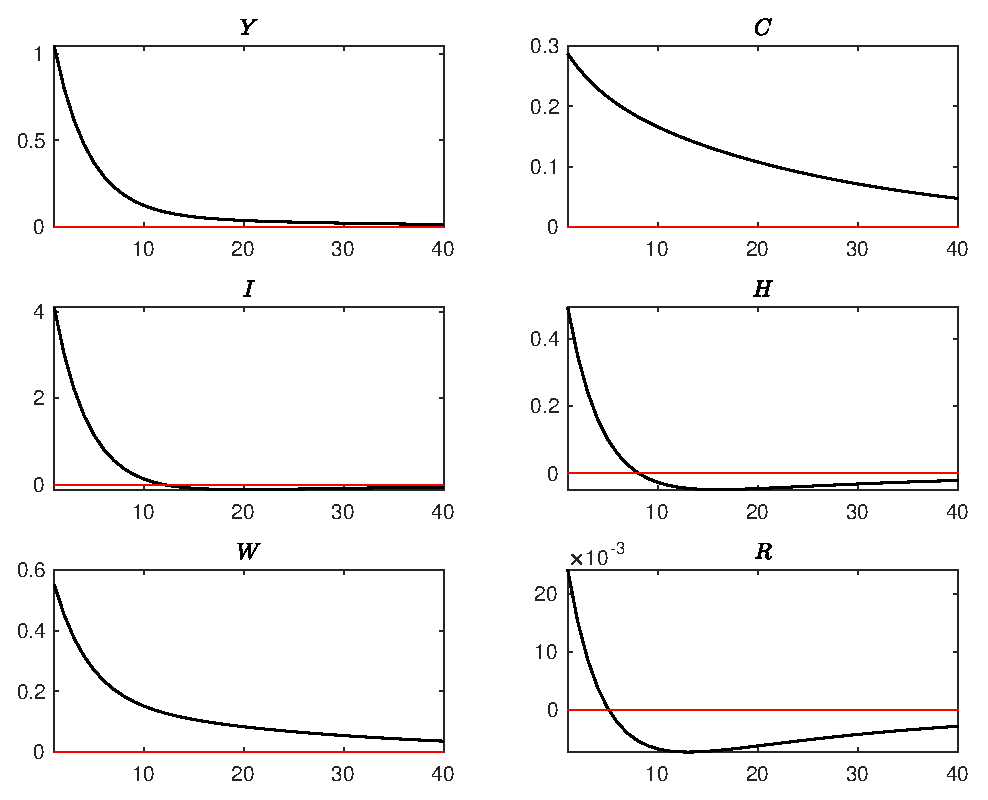
\includegraphics[width=0.80\textwidth]{RBClinear_basic/graphs/RBClinear_basic_IRF_epsA}
\caption{Impulse response functions (orthogonalized shock to ${\epsilon^{A}}$).}
\label{Fig:IRF:epsA}
\end{figure}
 
\begin{figure}[H]
\centering 
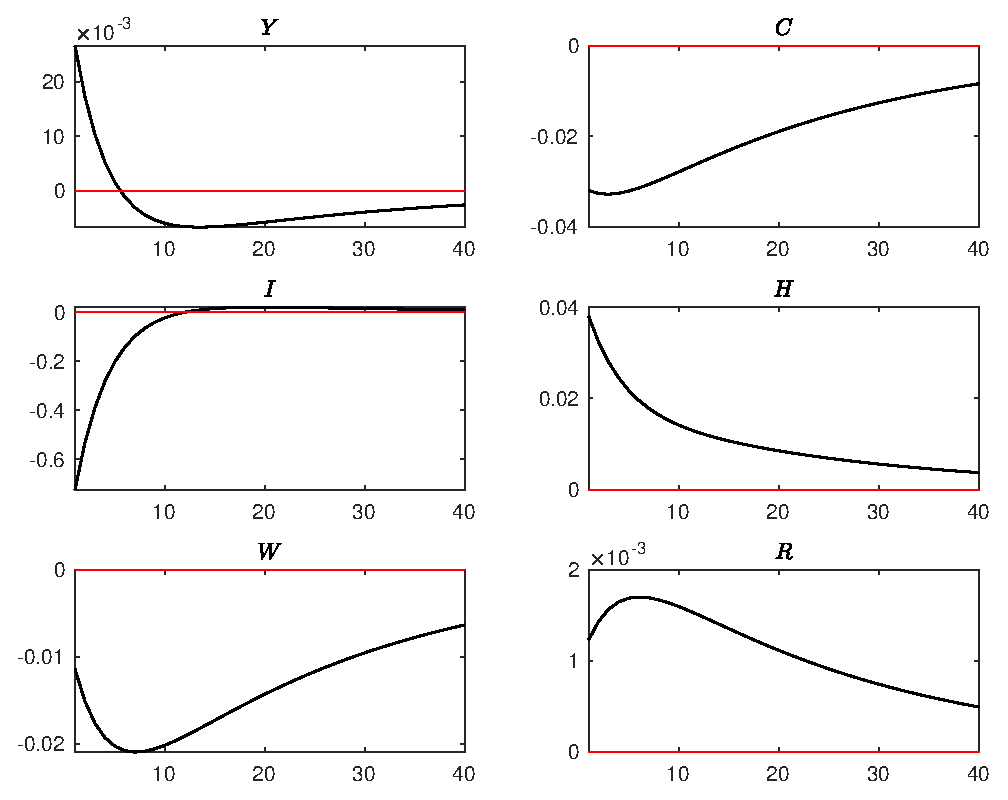
\includegraphics[width=0.80\textwidth]{RBClinear_basic/graphs/RBClinear_basic_IRF_epsG}
\caption{Impulse response functions (orthogonalized shock to ${\epsilon^{G}}$).}
\label{Fig:IRF:epsG}
\end{figure}
 
 
% End Of TeX file. 
 
\end{document} 
